\documentclass[10pt]{beamer}

\usetheme{metropolis}           % Use metropolis theme

\usepackage{minted}
\usepackage{tikz}
\usepackage{amsmath,mathpazo}

\usetikzlibrary{mindmap}

\title{DigitStringDiv1 \-- SRM 741, D1, 250-Pointer}

\author{Austin Jones}
\institute{University of Tennessee \-- Knoxville}

\date{\today}

\begin{document}

\maketitle

\begin{frame}{Overview}
  \Large
  \tableofcontents
\end{frame}

\section{Problem Intro}

\begin{frame}[fragile]{Statement and Constraints}
  \begin{minted}{cpp}
    class DigitStringDiv1 {
      public:
        long long count(string s, int x);
    };
  \end{minted}
  \begin{itemize}
    \item \textbf{Count the number of substrings of S that are greater than X.}
    \item Given: S, string containing characters from '0' through '9' and is at most 47 characters in length.
    \item Given: X, integer between 0 and 777,444,111.
    \item A substring of S is a string that results when you erase some subset of indices of S.
    \item A substring of S does not start with '0'.
    \item e.g. S is ``12356'', ``13'' and ``256'' are substrings. ``61'' is not.
  \end{itemize}
\end{frame}

\begin{frame}{Example 1}
  \Large
  $S = 101; X = 9 \rightarrow Answer = 3$ \\
  \begin{itemize}[<+->]
    \item $101$ \only<5->{$ > 9$}   \only<6>{Here!}
    \item $10$  \only<5->{$ > 9$}   \only<6>{Here!}
    \item $11$  \only<5->{$ > 9$}   \only<6>{Here!}
    \item $1$   \only<5->{$ \le 9$}
  \end{itemize}
\end{frame}

\begin{frame}{Example 2}
  \Large
  $S = 471; X = 47 \rightarrow Answer = 2$ \\
  \begin{itemize}[<+->]
    \item $471 $ \only<8->{$> 47$  }  \only<9->{Here!}
    \item $47  $ \only<8->{$\le 47$}   \only<10>{\emph{Notably Not} Here!}
    \item $41  $ \only<8->{$\le 47$}
    \item $71  $ \only<8->{$> 47$  }   \only<9->{Here!}
    \item $4   $ \only<8->{$\le 47$}
    \item $7   $ \only<8->{$\le 47$}
    \item $1   $ \only<8->{$\le 47$}
  \end{itemize}
\end{frame}

\begin{frame}{Some symbology}
  \Large
  \begin{itemize} % [<+->]
    \item Let i, j be a value 0-indexing into strings.
    \item Let $X_{S}$ be stringified X.
    \item Let $X_{i}$ be the value of $X_{S}$  at index i.
    \item Let $S_{i}$ be the value of S at index i.
    \item Let $X_{D}$ be the count of digits in $X_{S}$.
    \item Let $S_{D}$ be the count of digits in S.
  \end{itemize}
\end{frame}

\section{Slow, Dumb Solution}

\begin{frame}{Power Set Enumeration}
  \Large
  \begin{itemize} % [<+->]
    \item Create the power set of the S string.
    \item Process sets, based on the digit counts of $S_i$ and X.
      \begin{itemize}
        \large
        \item Fewer digits than X, discard.
        \item More digits than X, it must be greater.
        \item The same number of digits as X, convert $S_i$ to an integer and compare.
      \end{itemize}
    \item Return count of greater substrings.
  \end{itemize}
\end{frame}

\begin{frame}{Running Time}
  \Large
  \begin{itemize} % [<+->]
    \item Create the power set: $O(S_{D}*2^{S_{D}})$
    \item Process elements of power set: $O(S_{D}) * O(2^{S_{D}})$
      \begin{itemize}
        \large
        \item Fewer digits, discard: $O(1)$
        \item More digits, it must be greater: $O(1)$
        \item Same number of digits, convert $S_i$ and compare: $O(S_{D})$
      \end{itemize}
    \item Total: $O(S_{D}*2^{S_{D}}) + O(S_{D}*2^{S_{D}}) = O(S_{D}*2^{S_{D}})$
  \end{itemize}
\end{frame}

\section{Plank's Fast, Smart Solution}

\begin{frame}{Symbology Refresher}
  \Large
  \begin{itemize} % [<+->]
    \item Let i, j be a value 0-indexing into strings.
    \item Let $X_{S}$ be stringified X.
    \item Let $X_{i}$ be the value of $X_{S}$  at index i.
    \item Let $S_{i}$ be the value of S at index i.
    \item Let $X_{D}$ be the count of digits in $X_{S}$.
    \item Let $S_{D}$ be the count of digits in S.
  \end{itemize}
\end{frame}

\begin{frame}{The Algorithm}
  \Large
  \begin{itemize} % [<+->]
    \item Count all substrings of S with more digits than X. \\
      % For each index in S, count all the substrings starting at that index with more digits than X.
    \item Count all substrings of S with the same number of digits as X. \\
      % For each index in S, look at all substrings equal in length to X.
  \end{itemize}
\end{frame}

\begin{frame}{Digits Greater}
  \large
  For each index in S s.t. $S_{i}$ is non-zero and $i > X_{D}$, count all the substrings starting at that index with more digits than X.
  \begin{itemize} % [<+->]
    \item At all indices greater than the number of digits in X perform:
      \begin{equation*}
        CountGreater(S_{i}) = \sum_{j = X_{D}}^{i} \binom{i}{j}
      \end{equation*}
    \item The sum goes to $i$ and not $i + 1$, as $S_{i}$ is fixed.
    \item Likewise, the sum starts at $X_{D}$ \-- one digit is already chosen.
  \end{itemize}
\end{frame}

\begin{frame}{Digits Greater: Running Time}
  \large
  \begin{itemize} % [<+->]
    \item For all $S_{i}$ s.t. $i > X_{D}$: $O(S_D - X_D)$ \footnote{The ``$- X_D$'' comes back up later.}
    \item Look at all substring lengths from $X_D$ to $i$: $O(S_D - X_D)$
    \item i choose j: $O(j) \rightarrow O(S_D)$
    \item Total: $O(S_D - X_D)*O(S_D - X_D)*O(S_D) = O((S_{D})(S_{D} - X_D)^{2})$
  \end{itemize}
\end{frame}

\begin{frame}{Digits Equal}
  \large
  For each index in S, look at all substrings equal in length to X.
  Recursively enumerate the rest of S to a depth of $X_{D}$. \\ \\
  Define a routine, $CountEqual(i,j)$, that will compare $S_{i}$ and $X_{j}$.
  \begin{itemize}
    \item On success, spawn $CountEqual(k, j + 1)$ for all k from i to $S_{D}$.
    \item Success of $CountEqual(i, X_{D})$ returns 1 as a valid substring has been found.
    \item Success is $S_{i} \ge X_{j}$ for $j \ne X_{D}$
    \item Success is $S_{i} > X_{j}$ for $j = X_{D}$
  \end{itemize}
\end{frame}

\begin{frame}{Disclaimer}
  \Huge \textbf{Warning: Hand-waving Ahead!}
\end{frame}

\begin{frame}{Digits Equal: Running Time}
  Let $T_{0}(d)$ be the time/work to run $CountEqual(i, d)$.
  $T_{0}(0)$ is the exit a condition.
  $T_{0}(0)$ is $O(1)$ multiplied by the levels that reach it. \\
  \begin{align*}
    T_{0}(X_{D}) &= S_{D}T(X_{D} - 1) \\
         &= S_{D}S_{D}T(X_{D} - 2) \\
         &= {S_{D}}^{3}T(X_{D} - 3) \\
         &= {S_{D}}^{X_{D}}T(0) \\
         &= O({S_{D}}^{X_{D}}) \\
  \end{align*}
  Let $T(S, X)$ be the time/work to run $CountEqual$ for the full string.
  To get all the sums, $S_{D}$ runs of $T(X_{D})$ are required, yielding:
  \begin{equation*}
    T(S, X) = O({S_{D}}^{X_{D} + 1}) \\
  \end{equation*}
  This calculation assumes all recursions reach the exit condition.
  Which would never happen.
\end{frame}

\begin{frame}{Total Running Time/Comparison}
  The total runtime for this algorithm is:
  \begin{equation*}
    T_{smart}(S, X) = O({S_{D}}^{X_{D} + 1} + (S_{D})(S_{D} - X_D)^{2})
  \end{equation*}
  Great improvement over:
  \begin{equation*}
    T_{dumb}(S, X) = O(S_{D}*2^{S_{D}}) + O(S_{D}*2^{S_{D}}) = O(S_{D}*2^{S_{D}})
  \end{equation*}
\end{frame}

\section{Findings}

\begin{frame}{Speeding up Digits Equal}
  \begin{itemize}
    \item Memoization: \\
      $CountEqual(i, j)$ can be memoized on i and j.
      Making recurring recursion calls free.
    \item Reverse Iteration: \\
      The thought here is that iterating backwards would fill up the Memoization Cache faster.
    \item Early Exit: \\
      If in a call of $CountEqual(i, j)$, $S_{i} > X_{j}$ is found, return:\\
      \begin{equation*}
        \binom{S_{D} - i}{X_{D} - j}
      \end{equation*}\\
  \end{itemize}
\end{frame}


\begin{frame}{Different Methods to the Problem}
  \begin{figure}[ht!]
    \centering
    \includegraphics[width=0.9\textwidth]{../figures/comparison.ps}
  \end{figure}
\end{frame}

\begin{frame}{Time vs S}
  \begin{figure}[ht!]
    \centering
    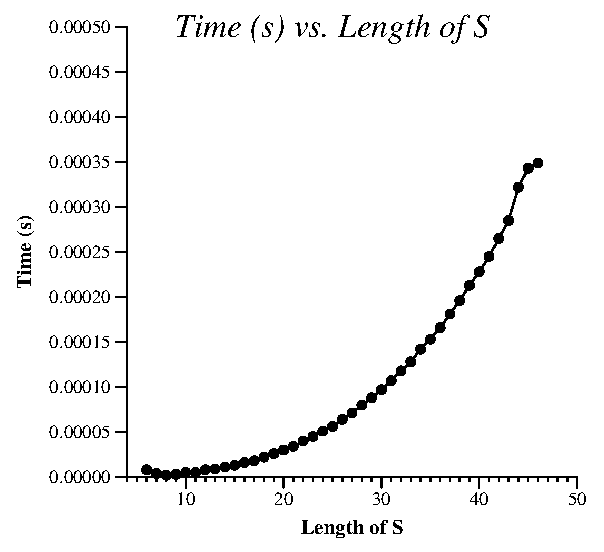
\includegraphics[width=0.9\textwidth]{../figures/vary_s.ps}
  \end{figure}
\end{frame}

\begin{frame}{Time vs X}
  \begin{figure}[ht!]
    \centering
    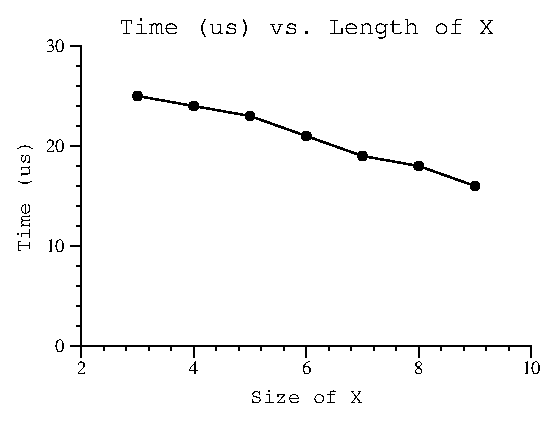
\includegraphics[width=0.9\textwidth]{../figures/vary_x.ps}
  \end{figure}
\end{frame}

\section{Wrapping Up}

\begin{frame}{Machine Specs}
  \Large
  MacBook Pro (15-inch, 2016)
  \begin{itemize} % [<+->]
    \item CPU\@: Intel i7\@-6700HQ (8) @ 2.60GHz
    \item GPU\@: AMD Radeon Pro 450
    \item Memory: 16384 MiB
  \end{itemize}

\end{frame}

\begin{frame}{How did Topcoder Do?}
  \large
  \begin{itemize}
    \item Problem Given in Topcoder: November, 2018
    \item Competitors who opened the problem: 99
    \item Competitors who submitted a solution: 82
    \item Number of correct solutions: 42
    \item Accuracy (percentage correct vs those who opened): 49.4\%
    \item Average Correct Time: 24.59
    \item Best Time: 4:56
  \end{itemize}
\end{frame}

\begin{frame}{Thank You}
  \Huge Questions?
\end{frame}

\end{document}

